\documentclass[11pt]{amsart}

% Margins
\usepackage[headheight=65pt]{geometry}
\geometry{
  top=1 in,
  inner=1 in,
  outer=1 in,
  bottom=1 in,
  headheight=3ex,
  headsep=2ex,
}

% Personal info, class, assignment
\def \fnamea{Dennis}
\def \fnameb{Neill}
\def \lnamea{Windham}
\def \lnameb{Shikada}
\def \class{CSCI 5448}
\def \hwnum{6} % Homework number
\def \assgn{Project \hwnum}
\newif\ifcode % Switch to toggle Python code insertion, see the end of the document for the value assignment

% Header
\usepackage{fancyhdr}
\pagestyle{fancy}
\lhead{\lnameb\ \& \lnamea}
\fancyfoot{}
\chead{\assgn}
\rhead{Page \thepage}
\renewcommand{\headrulewidth}{2pt}
%\renewcommand{\footrulewidth}{1pt}
\usepackage{pdflscape}


\usepackage{enumitem}
\usepackage{tabularx}
\usepackage{amssymb,amsmath,amsthm,amscd,mathrsfs,graphicx,color,pdfpages}
\usepackage[cmtip,all,matrix,arrow,tips,curve]{xy}
\usepackage[active]{srcltx}
\usepackage{mathpazo}
\usepackage{setspace}\doublespacing 
%Double space, and make it easier for the grader to grade your homework.
\usepackage{hyperref}
\usepackage[usenames,dvipsnames]{xcolor}
\usepackage[style=science,sortcites=true,sorting=nyt,backend=biber]{biblatex}
\hypersetup{colorlinks=true,citecolor=ForestGreen,linkcolor=Maroon,urlcolor=NavyBlue}

% Python raw code insertion
\usepackage{listings}
\usepackage{color}

% Python linting settings
\definecolor{dkgreen}{rgb}{0,0.6,0}
\definecolor{gray}{rgb}{0.5,0.5,0.5}
\definecolor{mauve}{rgb}{0.58,0,0.82}
\lstset{frame=tb,
  language=Python,
  aboveskip=3mm,
  belowskip=3mm,
  showstringspaces=false,
  columns=flexible,
  basicstyle={\small\ttfamily},
  numbers=none,
  numberstyle=\tiny\color{gray},
  keywordstyle=\color{blue},
  commentstyle=\color{dkgreen},
  stringstyle=\color{mauve},
  breaklines=true,
  breakatwhitespace=true,
  tabsize=3
}

% References
\addbibresource{./references.bib}

% Allows vertical lines in matrices like in tables
% Usage:
% \begin{bmatrix}[cc|cc] ...
\makeatletter
\renewcommand*\env@matrix[1][*\c@MaxMatrixCols c]{%
  \hskip -\arraycolsep
  \let\@ifnextchar\new@ifnextchar
  \array{#1}}
\makeatother

\newcommand{\marg}[1]{\normalsize{{\color{blue}\footnote{{\color{blue}#1}}}{\marginpar[\vskip -.3cm {\color{blue}\hfill\thefootnote$\implies$}]{\vskip -.3cm{ \color{blue}$\impliedby$\thefootnote}}}}}

\newcommand{\qc}[1]{\marg{#1}}

\setlength\fboxsep{.3cm}
\setlength\fboxrule{.05cm}

% Custom boxes
\newcommand*{\boxedcolor}{orange}
\makeatletter
\renewcommand{\boxed}[1]{\textcolor{\boxedcolor}{%
  \fbox{\normalcolor\m@th$\displaystyle#1$}}}
\makeatother

\makeatletter
\newcommand{\boxedred}[1]{\textcolor{red}{%
  \fbox{\normalcolor\m@th$\displaystyle#1$}}}
\makeatother

\makeatletter
\newcommand{\boxedblue}[1]{\textcolor{blue}{%
  \fbox{\normalcolor\m@th$\displaystyle#1$}}}
\makeatother

% Begin Document
\begin{document}

%region Author, Title, Abstract, TOC
\author[\lnamea]{\fnamea\ \lnamea\\\fnameb\ \lnameb}
\date{\today}
\title[\assgn]{\assgn \\ \ \\\class}
\maketitle
\tableofcontents
%endregion

\newpage
\section*{\textbf{Status Summary}}
\subsection*{Title}
\begin{center}
    \textit{Object Oriented Civilization Game Clone}
\end{center}

\subsection*{Team Members} \phantom{}

\begin{table}[htbp]
    \begin{tabularx}{\textwidth}{l|l|l}
        \textbf{Name}    & \textbf{Role}    & \textbf{Email}                  \\
        \hline
        Neill Shikada    & Graduate Student & Neill.Shikada@colorado.edu
        \\
        Dennis Windham   & Graduate Student & dene5275@colorado.edu           \\
        Bruce Montgomery & Instructor       & bruce.r.montgomery@colorado.edu
    \end{tabularx}
\end{table}

\subsection*{Work Done}
\begin{itemize}
    \item \textbf{Neill Shikada}
          \begin{itemize}
              \item Implemented complete AI that plays the game against other AI-controlled civilizations.
              \item Created UI using Unity's systems.
              \item Added audio support with royalty-free, copyright-free sound effects and music.
          \end{itemize}
    \item \textbf{Dennis Windham}
          \begin{itemize}
              \item Implemented board generation for the game.
              \item Implemented unit, behaviors, unit types, civilization types.
              \item Implement factories, graphics observer.
          \end{itemize}
\end{itemize}


\subsection*{Changes of Issues Encountered}

Unity generally advises tight coupling with their MonoBehavior base class, which is the only way to interact with the actual Unity object representations. We are avoiding MonoBehavior entirely for the underlying game logic, so we had to come up with a few workarounds when it comes to code interaction with Unity itself, e.g. a designated adapter-like helper class that does inherit from MonoBehavior. It was also initially unclear how we would facilitate graphics generation, but over a number of design iterations we decided to make use of the Observer pattern.

\newpage
\subsection*{Patterns}
\begin{itemize}
    \item Strategy
    \begin{itemize}
        \item We make heavy use of the strategy pattern to dynamically assign behaviors to Unit objects.
    \end{itemize}

    \item Factory
    \begin{itemize}
        \item We have multiple factories in place to generate various game objects. Namely, factories create individual Civilizations, Units and all Graphics objects.
    \end{itemize}

    \item Command
    \begin{itemize}
        \item We are using the Command pattern to bridge UI buttons with in-game actions for the human user.
    \end{itemize}

    \item Observer
    \begin{itemize}
        \item The Observer pattern is being used to update the visual representation of the game board. Whenever an object with a graphical representation spawns or gets destroyed the respective graphics observer is notified and performs an update.
    \end{itemize}

    \item Singleton 
    \begin{itemize}
        \item Singleton is being used for the persistent game settings object passed between scenes.
        \item GraphicsObserver is also implemented as a singleton so as to enforce its role as the only object that interacts with Unity graphics.
    \end{itemize}
\end{itemize}

\subsection*{Class Diagram} \phantom{}

See \hyperref[sec:appendixa]{Appendix A: Demonstration Class Diagram} for our class diagram.


\subsection*{Plan for Next Iteration} \phantom{}

We'll implement user controls, an actual turn-based system and endgame scoring. We expect to spend another 10-15 hours to complete the project.


% create a new page with special dimensions, include diagram
\newpage
\paperwidth=30in
\paperheight=20in
\pdfpagewidth=\paperwidth
\pdfpageheight=\paperheight

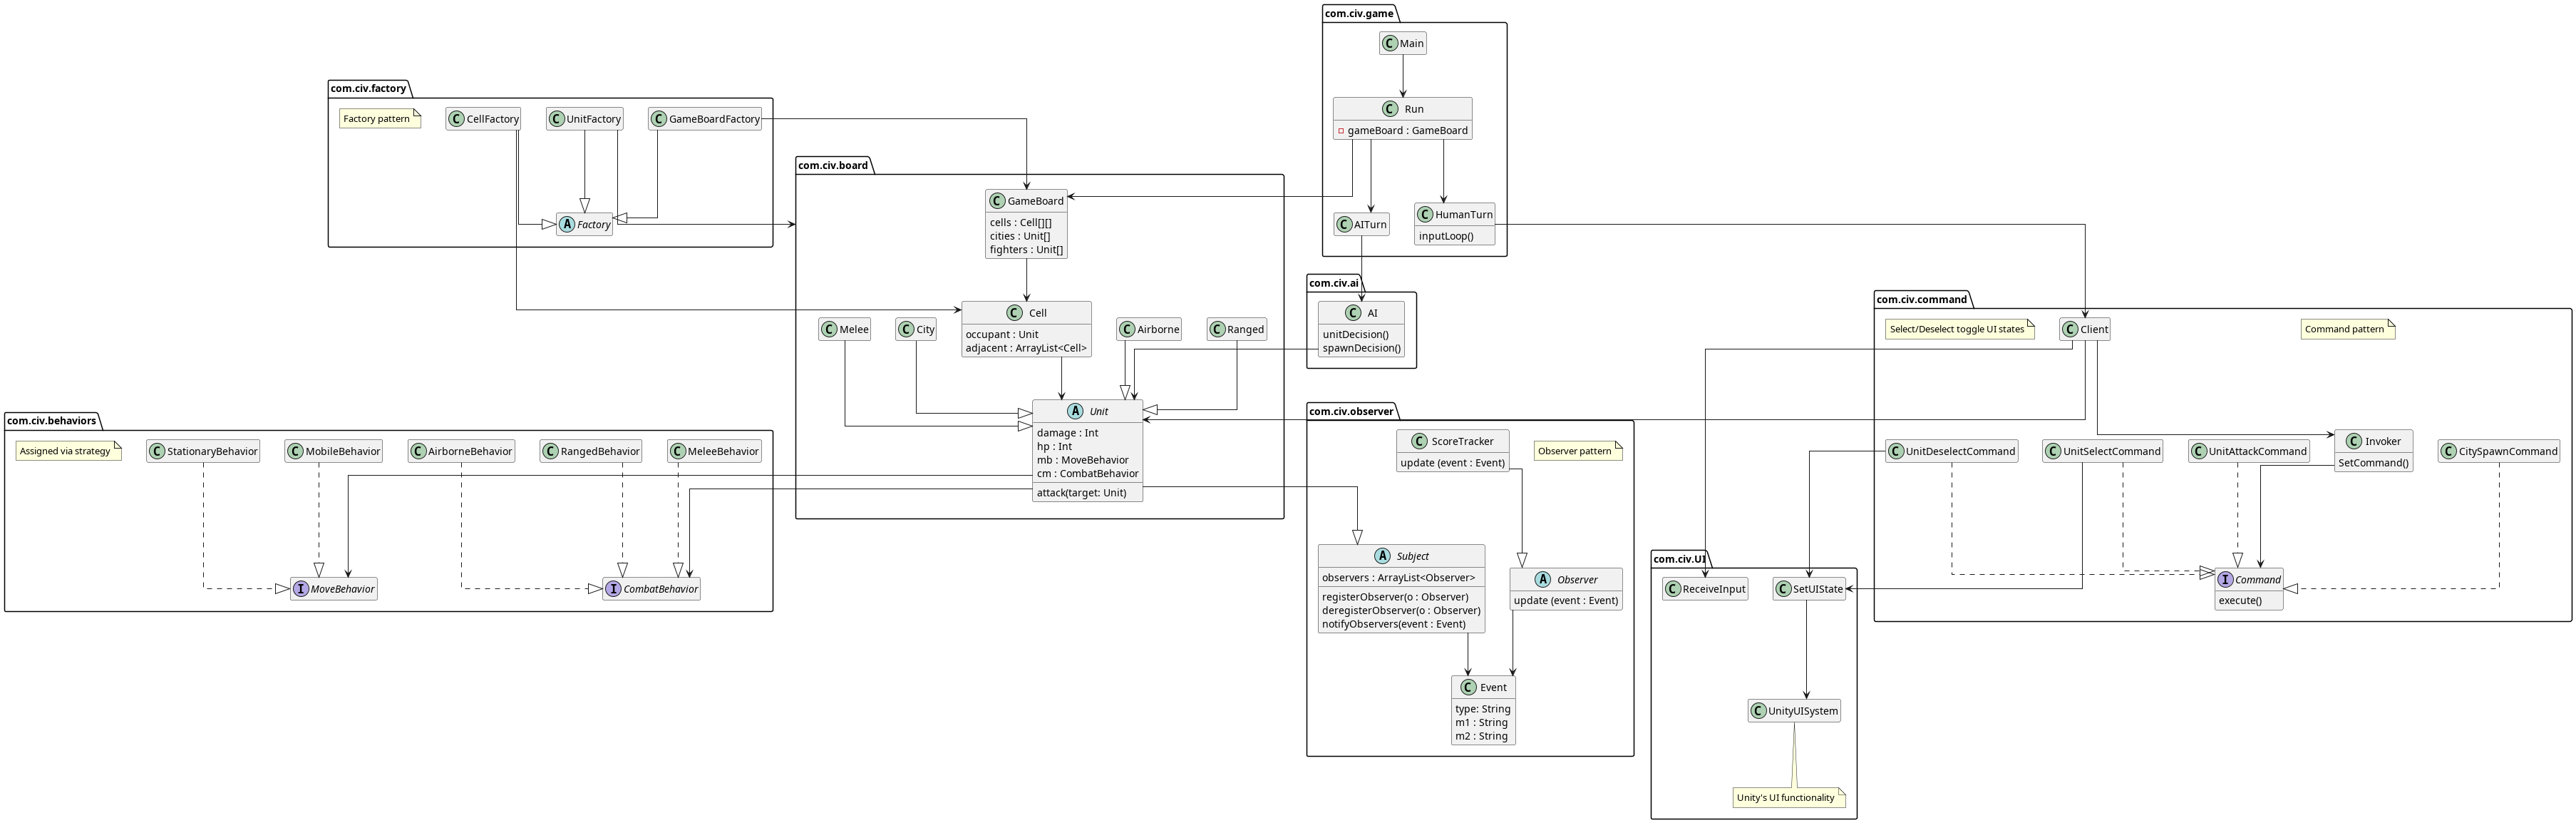
\includepdf[scale=0.9, offset=0mm 0mm, pagecommand={\section*{Appendix A: Demonstration Class Diagram}\pagestyle{fancy}}\label{sec:appendixa}]{../diagrams/class/class.png}


%\codetrue % Uncomment to enable code insertion
\ifcode
    % Python code section, toggled by the switch above
    % The code file is expected to be follow the "hw{\hwnum}.py" naming convention
    \newpage
    \section*{Code}
    \label{sec:code}
    \lstinputlisting[language=Python]{Code/hw\hwnum.py}
\fi


% \includepdf[scale=0.98, pagecommand={\section*{Appendix A: Class Diagram for RotLA}\pagestyle{fancy}}\label{sec:appendixa}]{../uml/game_diagram.png}


\end{document}
